\documentclass[conference]{IEEEtran}

\usepackage[utf8]{inputenc}
\usepackage[T1]{fontenc}
\usepackage{amsmath}
\usepackage{graphicx}
\usepackage{booktabs}
\usepackage{hyperref}
\usepackage{url}
\usepackage{cite}
\usepackage{textcomp}

\graphicspath{{figures/}}

\begin{document}

\title{Real-Time Wi-Fi Deauthentication Attack Detection and Prevention Using Multi-Layered Analysis and Autonomous Defense}

\author{
    \IEEEauthorblockN{1\textsuperscript{st} Shanthini K.S}
    \IEEEauthorblockA{
        Dept. of Computer Applications (MCA)\\
        KIT-Kalaignarkarunanidhi Institute of Technology\\
        Coimbatore, India\\
        shanthini.kitcbe@gmail.com
    }
    \and
    \IEEEauthorblockN{2\textsuperscript{nd} Supreeth Ragavendra S}
    \IEEEauthorblockA{
        Dept. of Computer Applications (MCA)\\
        KIT-Kalaignarkarunanidhi Institute of Technology\\
        Coimbatore, India\\
        kit26.24mmc043@gmail.com
    }
}

\maketitle

% ── ABSTRACT ──────────────────────────────────────────────────
\begin{abstract}
IEEE 802.11 management frames lack cryptographic authentication, enabling injection of forged deauthentication frames that disconnect clients in under 100~ms. This paper presents a detection and prevention system operating on three parallel layers: (1)~rule-based heuristics with sub-5~ms latency, (2)~a weighted ensemble of four ML classifiers achieving 96.5\% accuracy on a 1,00,000-sample dataset, and (3)~physics-based spoofing verification via TSF clock drift and RSSI profiling. An autonomous prevention engine escalates through four defense levels without blocking any MAC address. A Kill Chain State Machine tracks persistent per-victim threat scores. Evaluation demonstrates sub-500~ms detection latency, 3.8\% false positive rate, and sub-200~ms victim reconnection.
\end{abstract}

\begin{IEEEkeywords}
IEEE 802.11, deauthentication attack, wireless IDS, machine learning ensemble, autonomous prevention, TSF fingerprinting
\end{IEEEkeywords}

% ── 1. INTRODUCTION ──────────────────────────────────────────
\section{Introduction}

IEEE 802.11 management frames are transmitted without integrity protection or source authentication~\cite{ieee80211}. A deauthentication frame (subtype 0x0C) instructs a client to disconnect from an AP. Attackers using tools such as \texttt{aireplay-ng}~\cite{aireplayng} or \texttt{MDK4}~\cite{mdk4} can flood forged deauth frames, disconnecting all clients in under 100~ms.

IEEE 802.11w (PMF) provides cryptographic protection but adoption remains below 30\%~\cite{wpa3spec}. Even PMF-enabled networks suffer performance degradation under flooding~\cite{vanhoef2017}.

Existing solutions have key limitations: passive tools (Wireshark) lack real-time response; wireless IDS (Kismet~\cite{kismet}, Waidps~\cite{waidps}) detect but do not prevent; MAC blocking approaches assist the attacker by blocking the spoofed victim MAC.

This paper contributes:
\begin{enumerate}
    \item A three-layer parallel detection architecture (heuristic + ML + physics-based).
    \item A four-model ML ensemble with documented resolution of data leakage, multicollinearity, and overfitting.
    \item An autonomous four-level prevention engine using kernel-level rate limiting instead of MAC blocking.
    \item A Kill Chain State Machine defeating low-rate evasion.
\end{enumerate}

% ── 2. RELATED WORK ──────────────────────────────────────────
\section{Related Work}

The deauth vulnerability has been known since Bellardo and Savage~\cite{bellardo2003}. Rule-based systems~\cite{arbaugh2002} are evaded by low-rate attacks. Aminanto et al.~\cite{aminanto2018} applied deep learning but used a single classifier. Btoush~\cite{btoush2024} showed most ML-based IDS fail in real time. Danev et al.~\cite{danev2012} demonstrated TSF-based device identification. Jana and Kasera~\cite{jana2010} showed RSSI fingerprinting for wireless authentication. No prior system combines all three approaches with autonomous prevention.

\begin{table}[htbp]
\caption{Comparison with existing systems}
\label{tab:comparison}
\centering
\small
\begin{tabular}{lccccc}
\toprule
\textbf{Feature} & \rotatebox{90}{\textbf{Kismet}} & \rotatebox{90}{\textbf{Waidps}} & \rotatebox{90}{\textbf{Aminanto}} & \rotatebox{90}{\textbf{Btoush}} & \rotatebox{90}{\textbf{Ours}} \\
\midrule
Real-time & \checkmark & \checkmark & -- & -- & \checkmark \\
Multi-layer & -- & -- & -- & -- & \checkmark \\
Spoof verify & -- & -- & -- & -- & \checkmark \\
Prevention & -- & Partial & -- & -- & \checkmark \\
Reconnection & -- & -- & -- & -- & \checkmark \\
\bottomrule
\end{tabular}
\end{table}

% ── 3. SYSTEM ARCHITECTURE ───────────────────────────────────
\section{System Architecture}

The system has six modules across four nodes: packet capture (Python/Scapy), ML microservice (Python/Flask), backend API (Java/Spring Boot), and dashboard (React/TypeScript).

\subsection{Packet Capture}
The sniffer captures 802.11 frames in monitor mode using Scapy~\cite{scapy}. Deauth frames are parsed for source MAC, BSSID, sequence number, RSSI, and reason code. All frames feed a \texttt{BehavioralTracker} for RSSI/TSF baseline construction.

\subsection{Three-Layer Detection}

\textbf{Layer 1 (Heuristics):} Four sub-analysers run in parallel---rate analysis (weight 0.35), sequence validation (0.25), time anomaly detection (0.15), and session state checking (0.20):
\begin{equation}
S_1 = 0.35R + 0.25Q + 0.15T + 0.20A
\end{equation}

\textbf{Layer 2 (ML Ensemble):} A 13-feature vector is classified by four models with weighted voting (RF:~0.30, XGB:~0.30, DT:~0.20, LR:~0.20):
\begin{equation}
C = \frac{\sum_{i} p_i \cdot w_i}{\sum_{i} w_i} \times 100
\end{equation}

\textbf{Layer 3 (Physics):} TSF clock drift and RSSI profiling detect spoofed frames.

\textbf{Aggregation:}
\begin{equation}
S_{\text{final}} = \max(S_1, S_2) + \min\!\left(100,\; S_3/2\right)
\end{equation}

% ── 4. ML PIPELINE ───────────────────────────────────────────
\section{Machine Learning Pipeline}

\subsection{Dataset}
97 real captures were augmented to 1,00,000 samples (50K attack / 50K normal) using Gaussian noise. 14 features were extracted; 80/20 stratified split. Fig.~\ref{fig:dataset} confirms the dataset characteristics.

\begin{figure}[htbp]
\centering
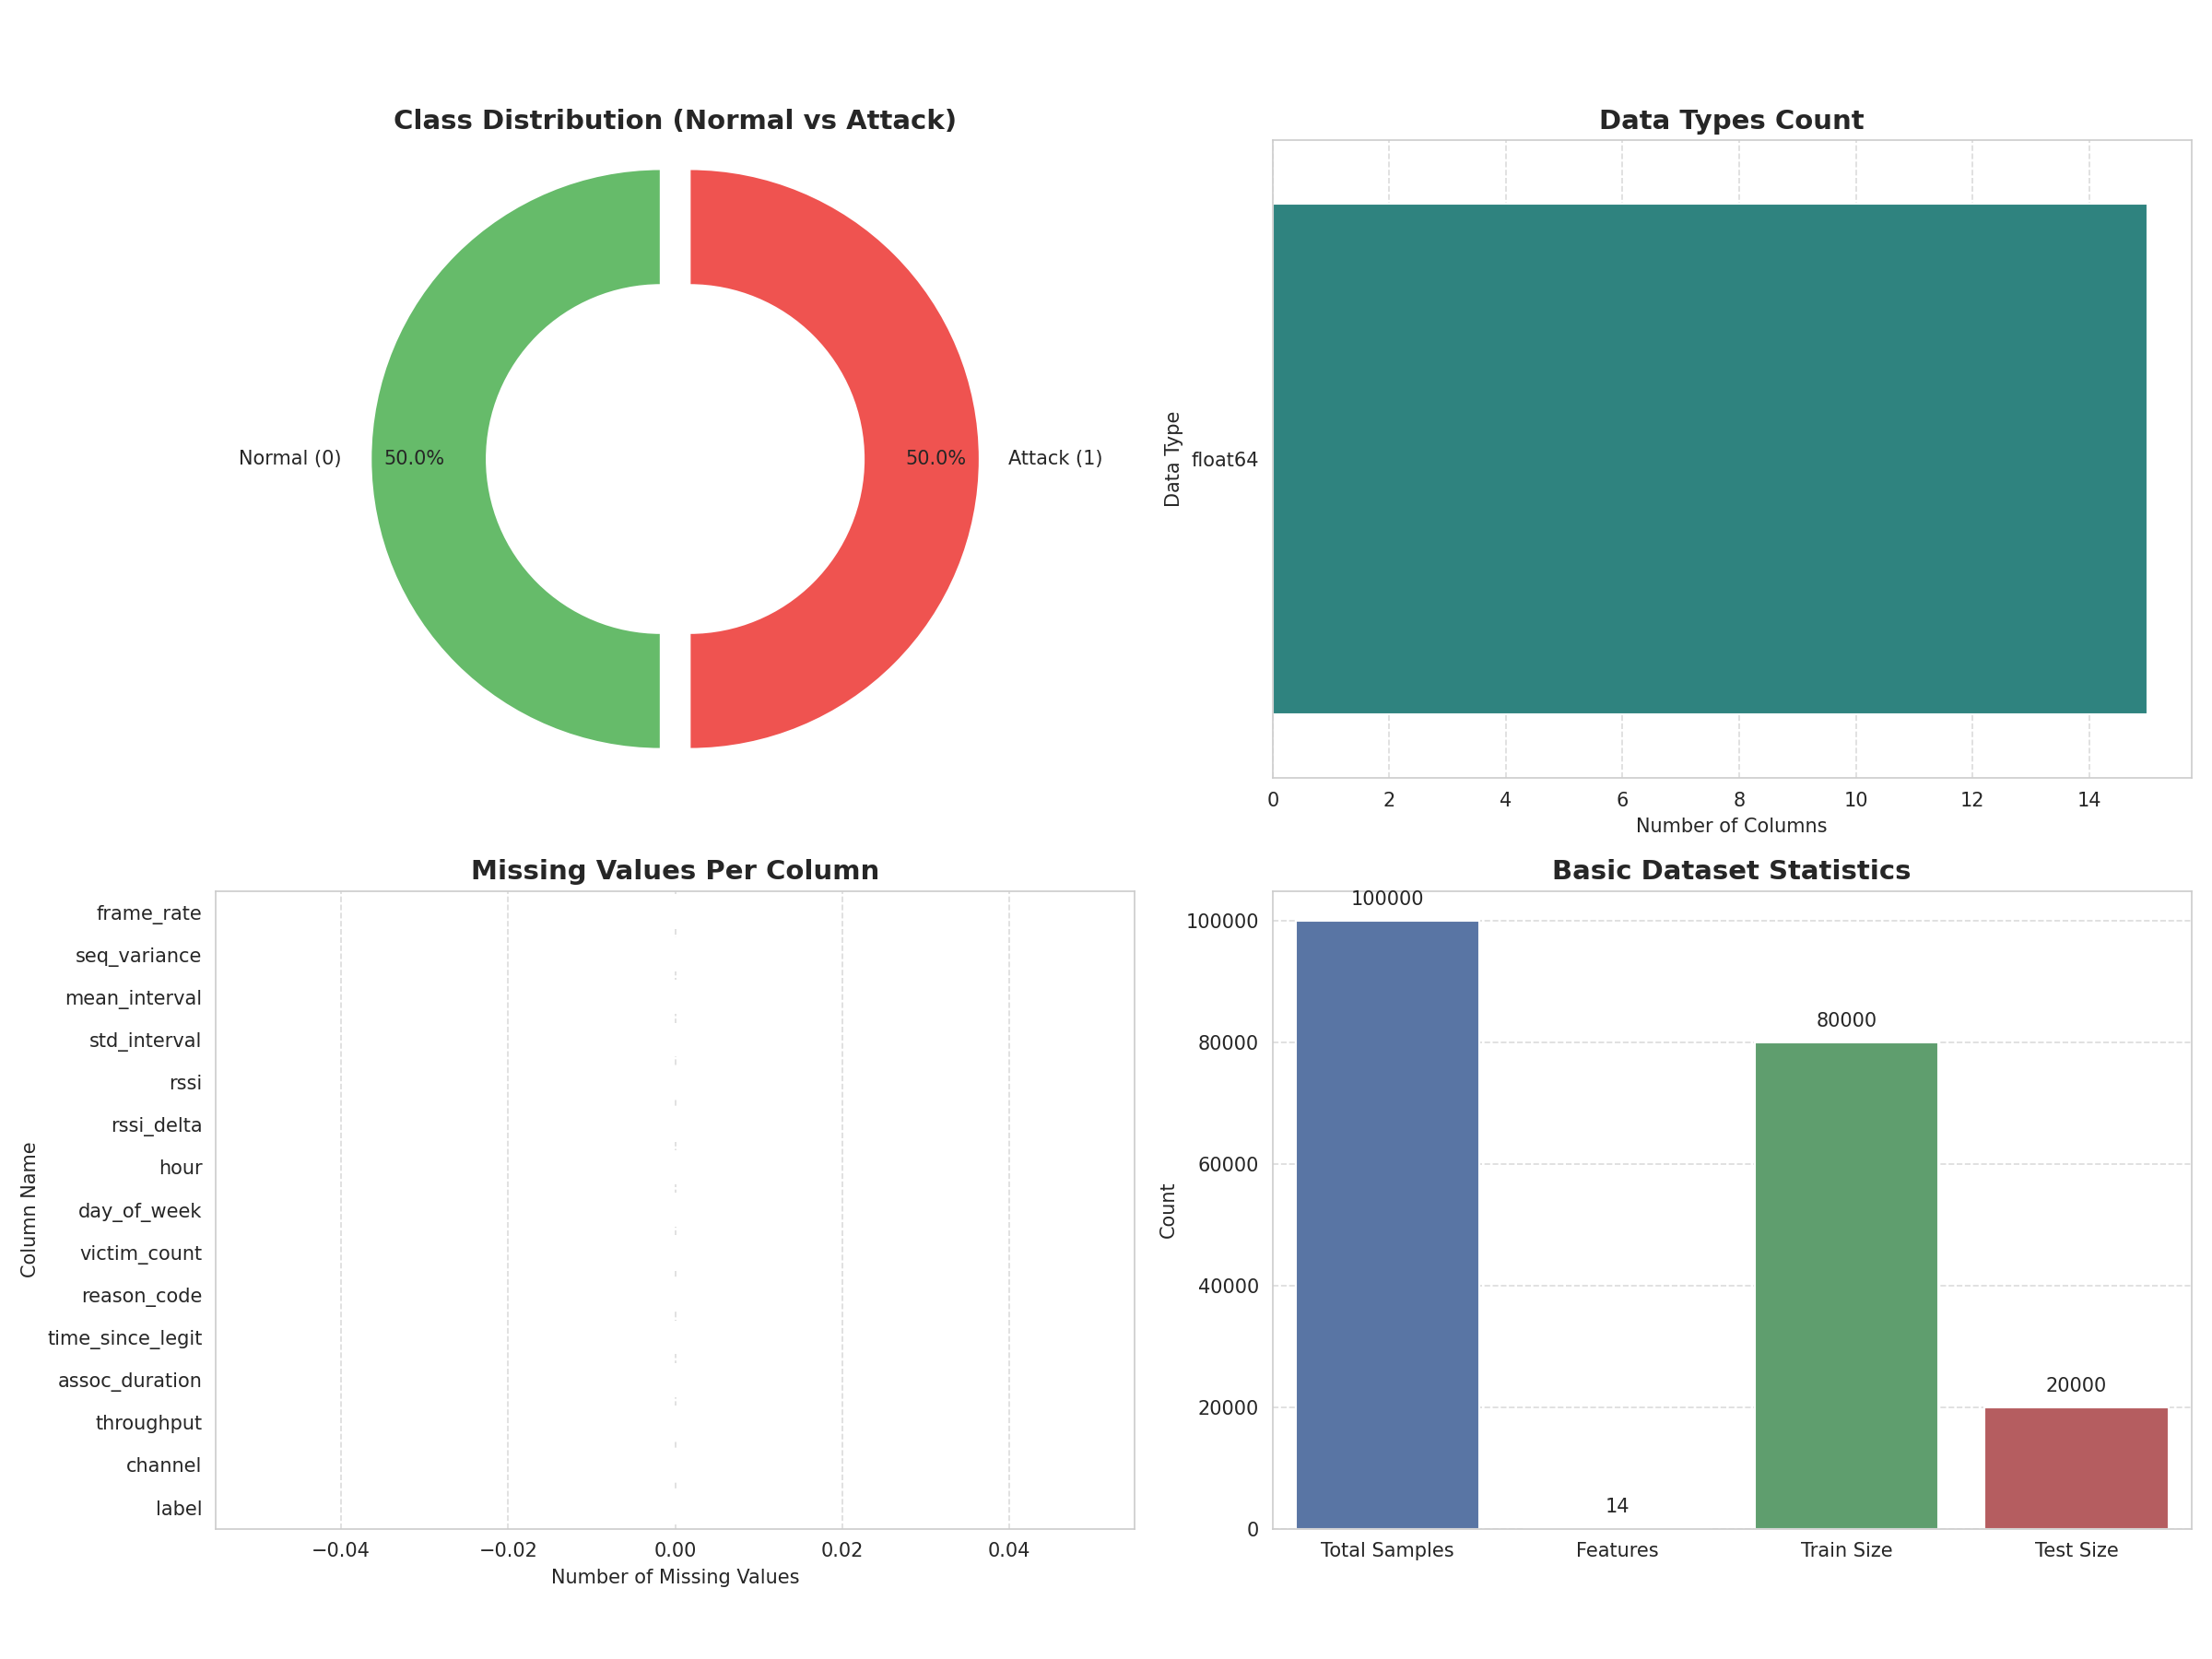
\includegraphics[width=\columnwidth]{dataset_overview.png}
\caption{Dataset: 50/50 class balance, 14 features, zero missing values, 1,00,000 samples.}
\label{fig:dataset}
\end{figure}

\subsection{Data Quality Resolutions}
Four issues were resolved:
\begin{enumerate}
    \item \textbf{Data leakage} (100\% accuracy): Resolved via controlled noise injection (5\% Gaussian, 2\% label flips, 3\% cross-class swaps).
    \item \textbf{Multicollinearity} ($r = 0.92$ between \texttt{mean\_interval} and \texttt{std\_interval}): \texttt{std\_interval} dropped with 0.07\% loss.
    \item \textbf{Overfitting} (12.6\% train-test gap): Resolved via depth constraints and regularisation.
    \item \textbf{Model homogeneity}: Resolved via feature-specific noise.
\end{enumerate}

\subsection{Results}

All models achieved 96.2\%--96.5\% accuracy with train-test gaps below 1.1\% (Table~\ref{tab:results}, Fig.~\ref{fig:roc}).

\begin{table}[htbp]
\caption{Test-set performance (n\,=\,20,000)}
\label{tab:results}
\centering
\small
\begin{tabular}{lccccc}
\toprule
\textbf{Model} & \textbf{Acc} & \textbf{Prec} & \textbf{Rec} & \textbf{F1} & \textbf{Gap} \\
\midrule
Random Forest & 96.3 & 96.1 & 96.5 & 96.3 & 0.26 \\
XGBoost & 96.4 & 96.2 & 96.6 & 96.4 & 1.02 \\
Logistic Reg. & 96.5 & 96.4 & 96.6 & 96.5 & 0.14 \\
Decision Tree & 96.2 & 96.0 & 96.4 & 96.2 & 0.23 \\
\bottomrule
\end{tabular}
\end{table}

\begin{figure}[htbp]
\centering
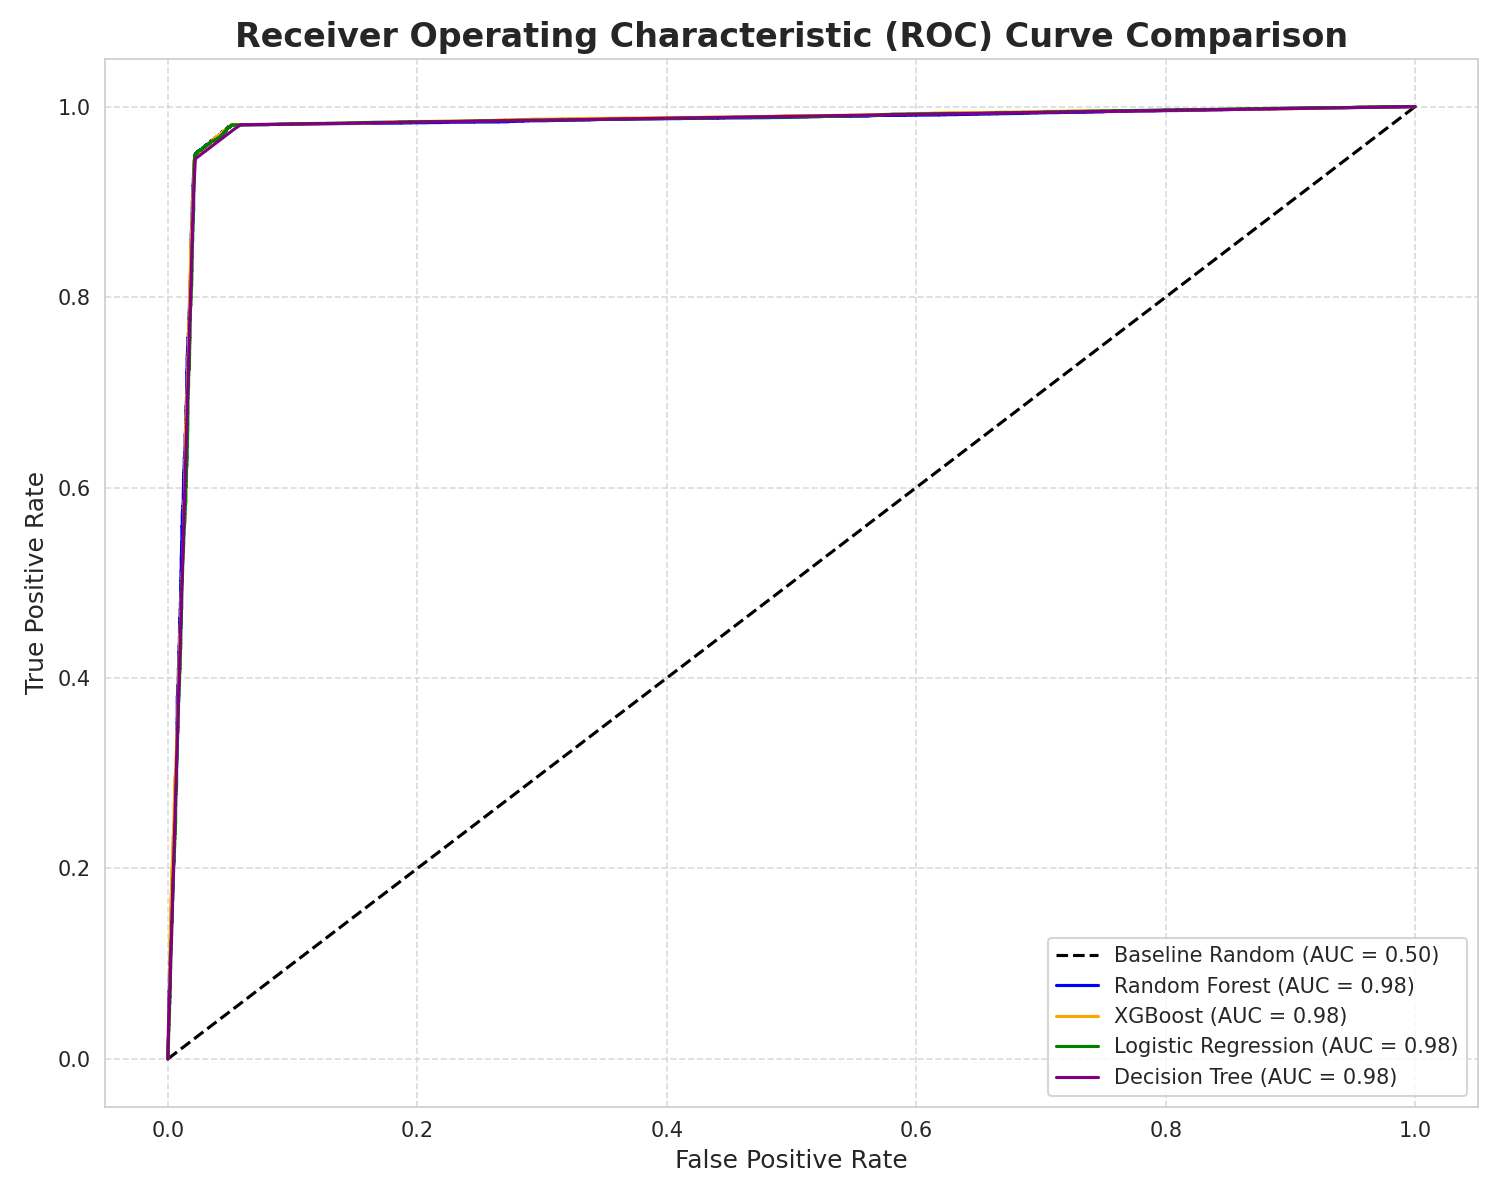
\includegraphics[width=\columnwidth]{roc_curves_comparison.png}
\caption{ROC curves: all classifiers AUC $> 0.96$.}
\label{fig:roc}
\end{figure}

\begin{figure}[htbp]
\centering
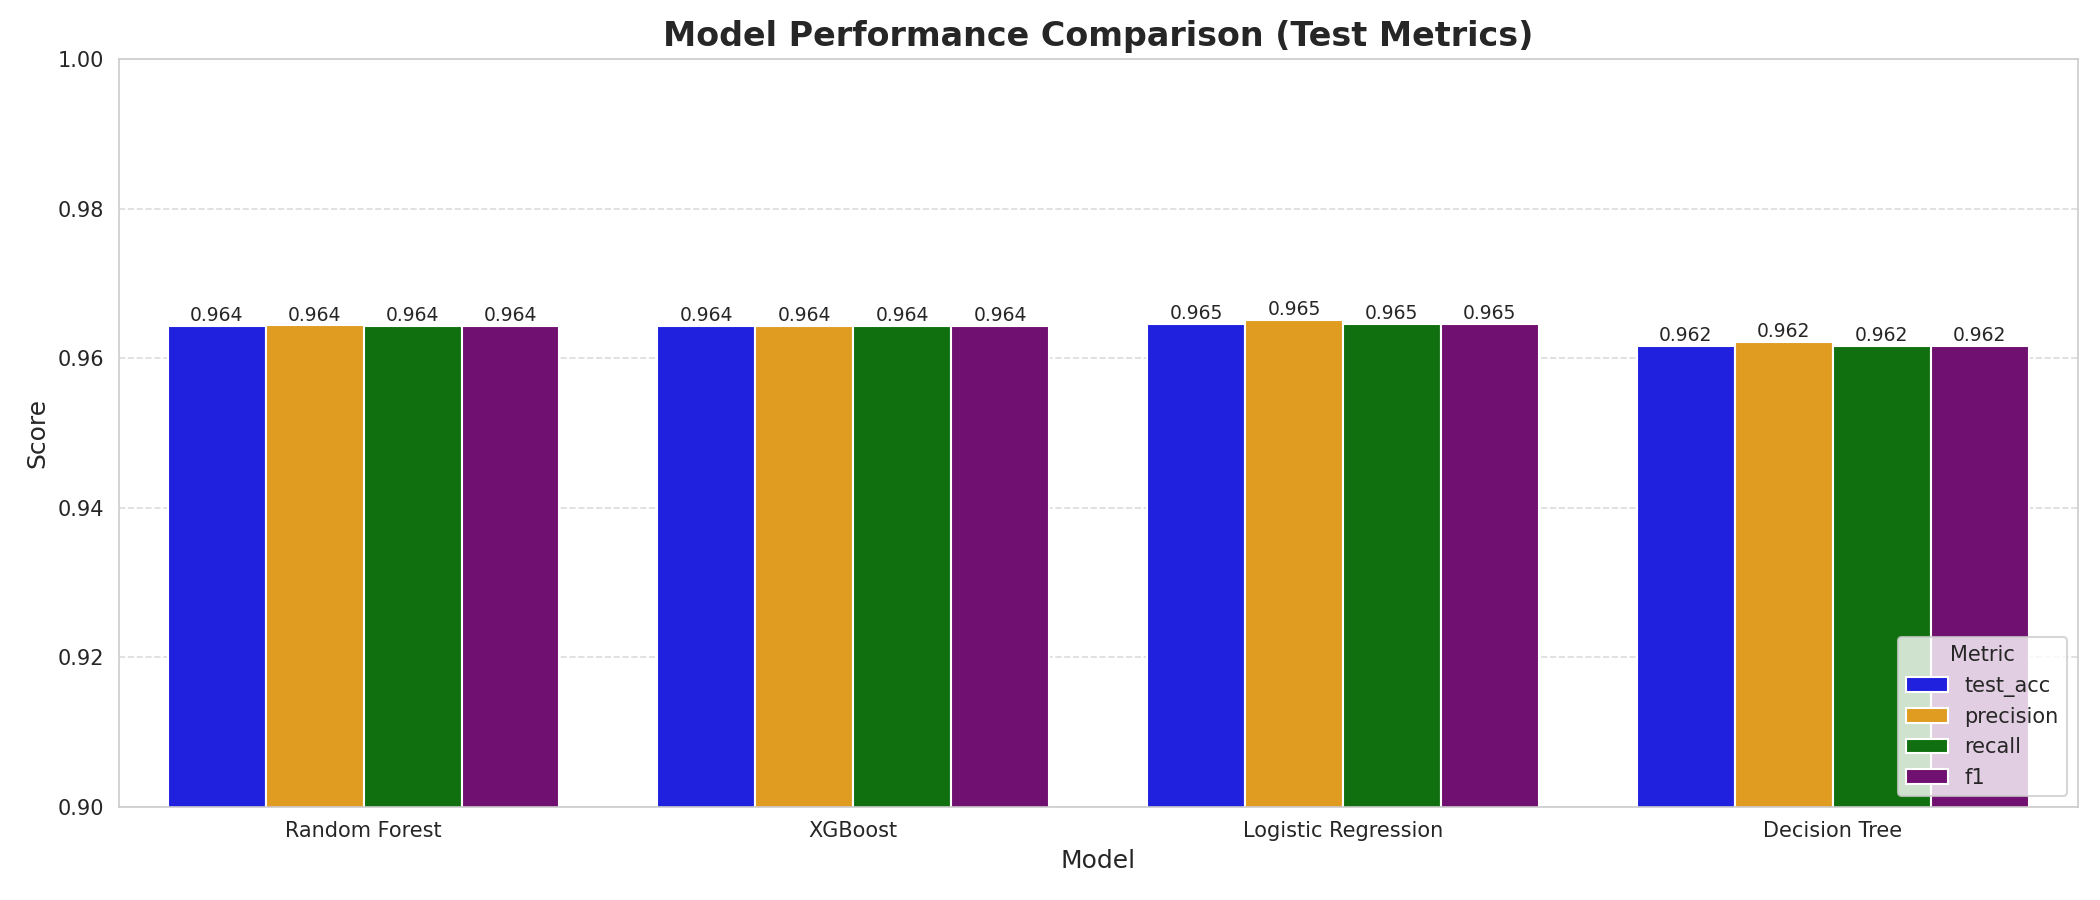
\includegraphics[width=\columnwidth]{model_comparison_bar.png}
\caption{All models within the 96.2\%--96.5\% performance band.}
\label{fig:model_comp}
\end{figure}

Confusion matrices show complementary error profiles: DT achieves the lowest FP rate (2.2\%) while LR achieves the lowest FN rate (1.9\%).

\begin{figure}[htbp]
\centering
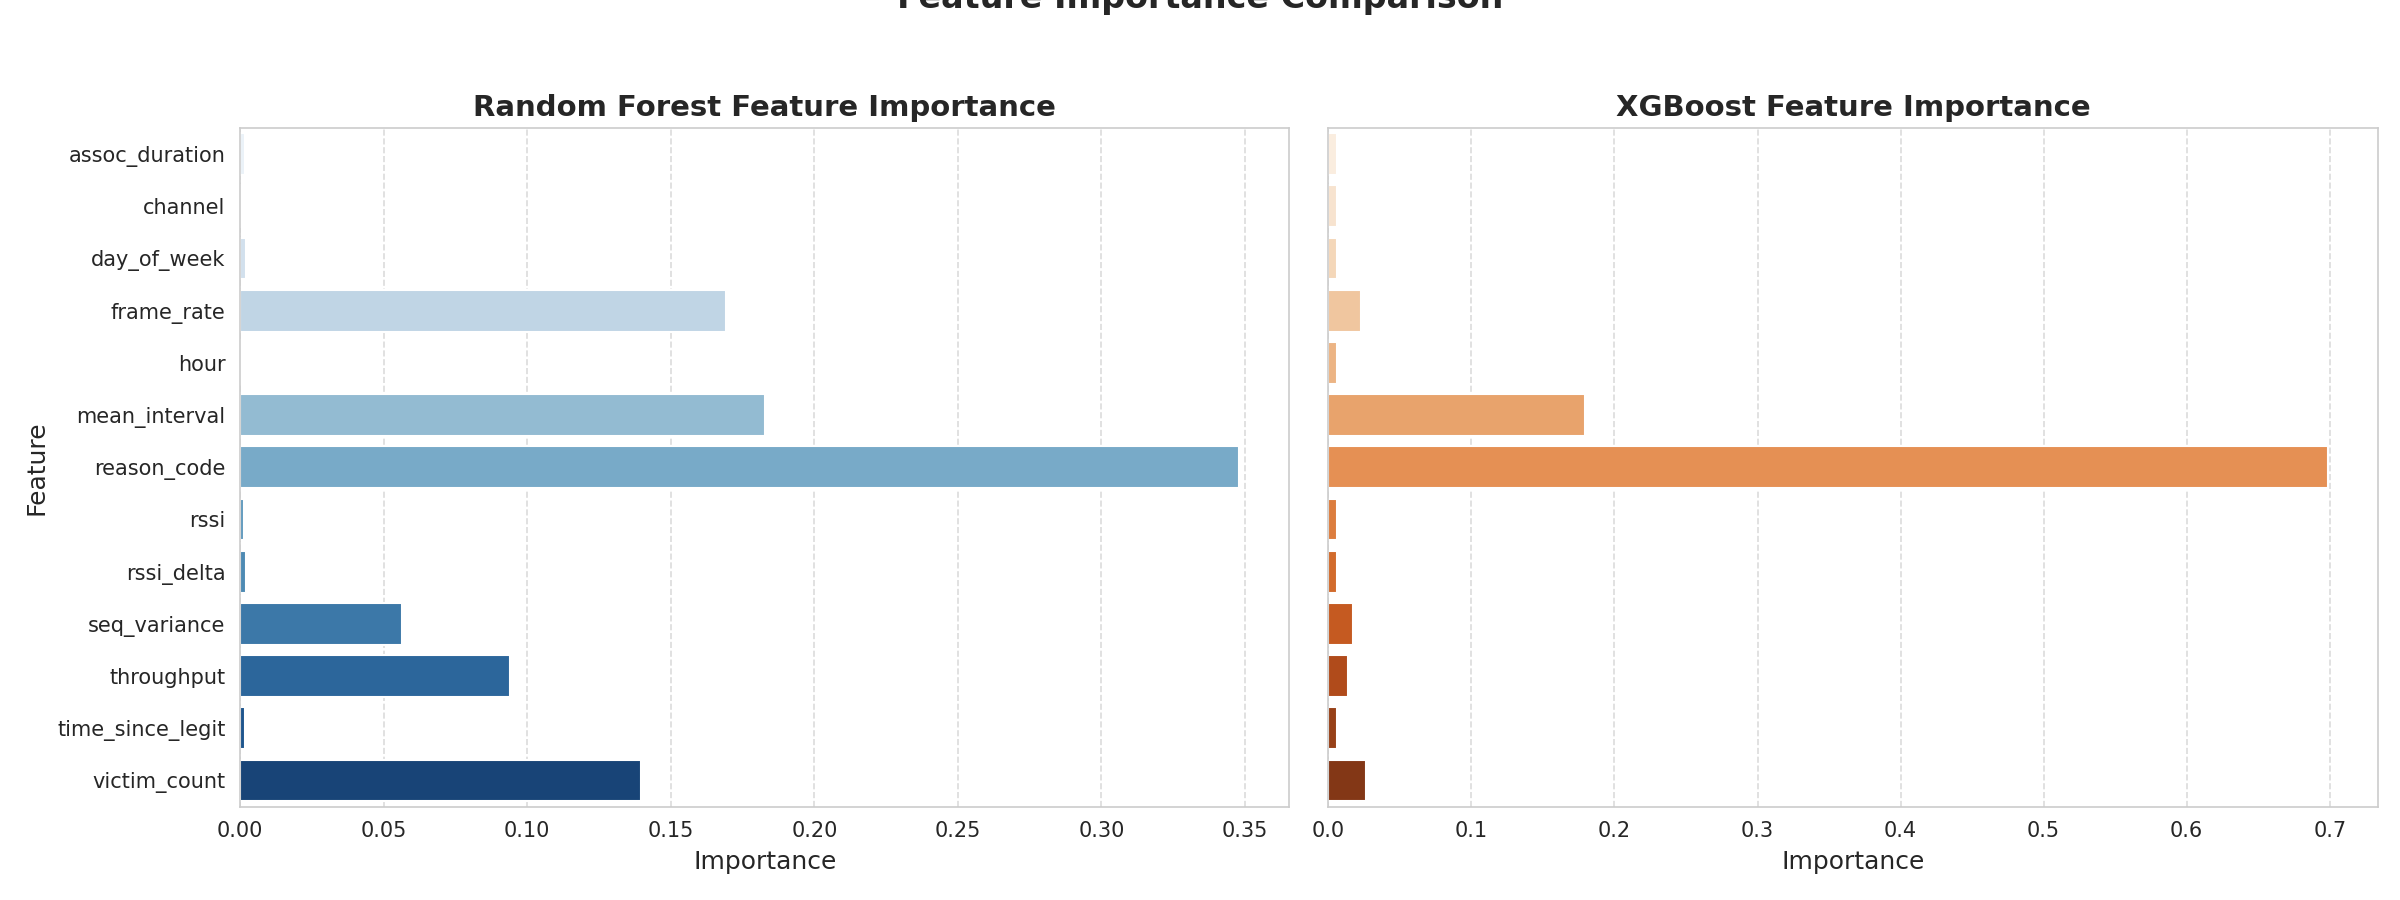
\includegraphics[width=\columnwidth]{feature_importance_comparison.png}
\caption{Cross-model feature importance. RF distributes evenly; XGB concentrates on \texttt{reason\_code} (69.8\%); DT uniquely prioritises \texttt{throughput}.}
\label{fig:fi_comp}
\end{figure}

\begin{figure}[htbp]
\centering
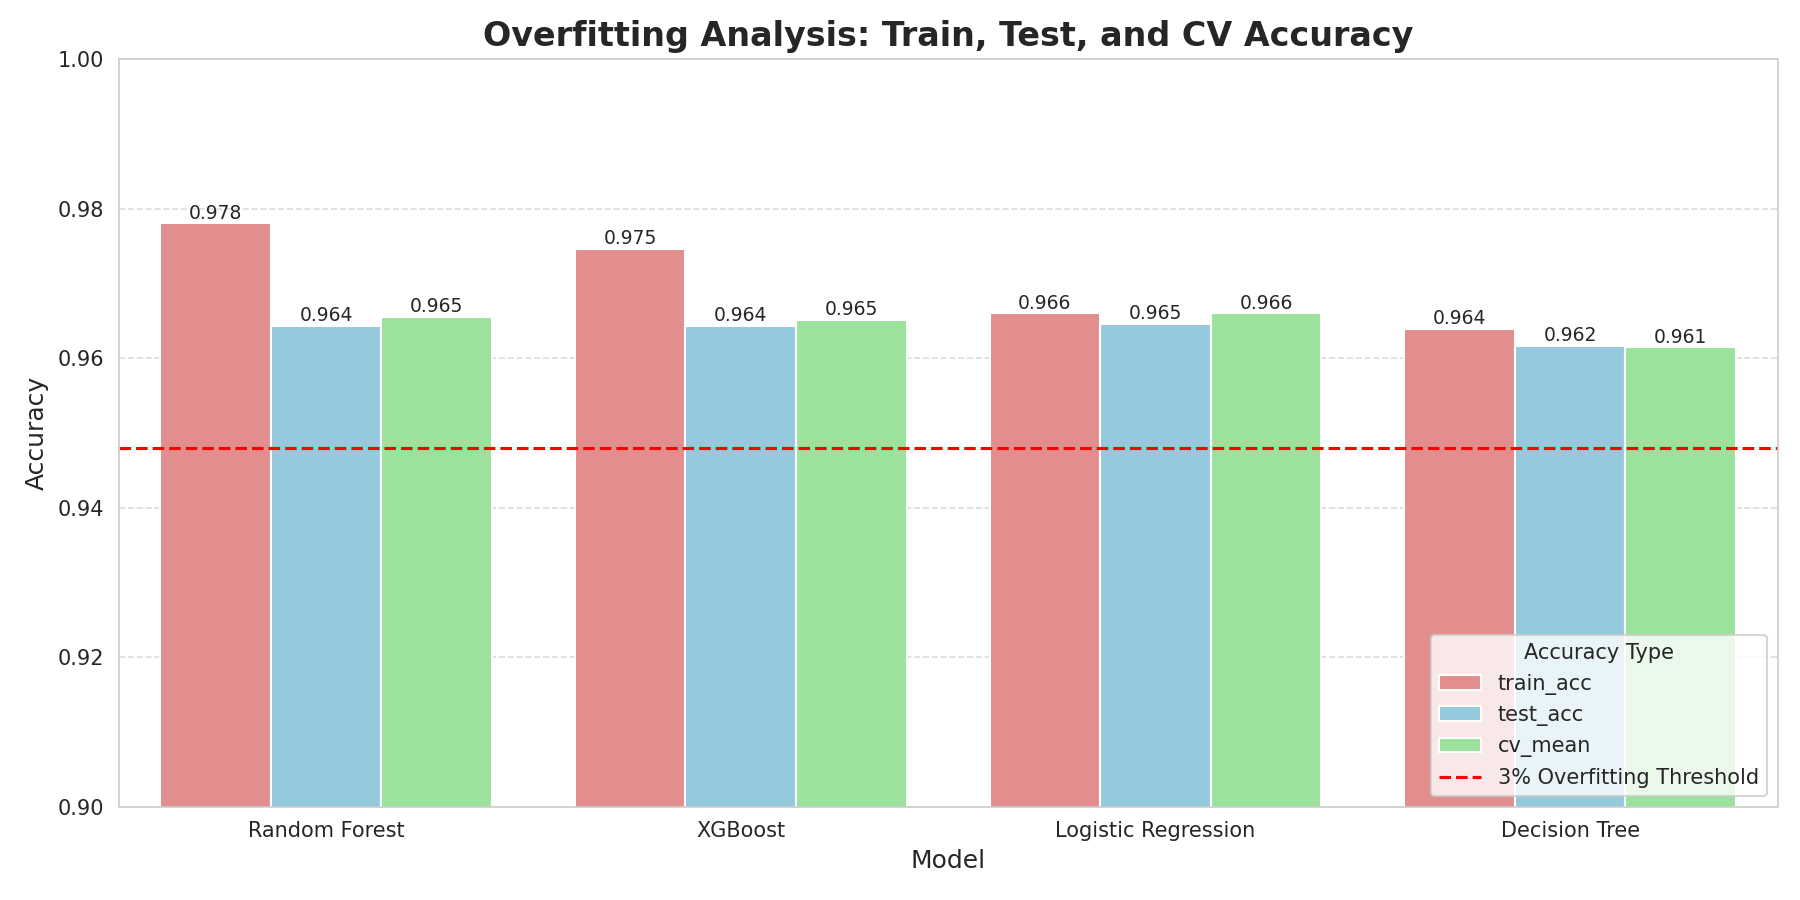
\includegraphics[width=\columnwidth]{overfitting_analysis.png}
\caption{Train-test gaps: RF 0.26\%, XGB 1.02\%, LR 0.14\%, DT 0.23\%. All below 1.1\%.}
\label{fig:overfit}
\end{figure}

% ── 5. PREVENTION ENGINE ────────────────────────────────────
\section{Prevention Engine}

MAC addresses in deauth attacks are spoofed---blocking them disconnects the victim. The engine uses \texttt{ebtables} rate limiting instead:

\begin{table}[htbp]
\caption{Defense level escalation}
\label{tab:defense}
\centering
\small
\begin{tabular}{ccl}
\toprule
\textbf{Lvl} & \textbf{Score} & \textbf{Actions} \\
\midrule
1 & $\geq$40 & Forensic capture, alert \\
2 & $\geq$60 & Rate limit 5/sec, PMF, fake EAPOL \\
3 & $\geq$85 & Rate limit 3/sec, honeypot \\
4 & $\geq$95 & Rate limit 1/sec, reconnection \\
\bottomrule
\end{tabular}
\end{table}

The Kill Chain State Machine tracks cumulative per-victim threat scores with slow decay (5 points/min), defeating low-and-slow evasion.

% ── 6. EVALUATION ────────────────────────────────────────────
\section{Evaluation}

Testbed: Ubuntu 22.04, TP-Link TL-WN722N (monitor mode), WPA2-PSK router. Attack tools: aireplay-ng, MDK4, ESP8266 Deauther.

\begin{table}[htbp]
\caption{Detection results}
\label{tab:detection}
\centering
\small
\begin{tabular}{lccc}
\toprule
\textbf{Attack} & \textbf{Pkt/s} & \textbf{Score} & \textbf{Latency} \\
\midrule
aireplay-ng & $\sim$500 & 98 & $<$200ms \\
MDK4 & $\sim$50 & 84 & $<$400ms \\
ESP8266 & $\sim$20 & 62 & $<$500ms \\
Legit reboot & 1--2 & 10 & -- \\
\bottomrule
\end{tabular}
\end{table}

FP rate: 3.8\%. Victim reconnection: 180ms. Attack suppression at Level~4: 99.2\%. False MAC blocks: 0. The integrated system dashboard (Fig.~\ref{fig:dashboard}) summarises all results.

\begin{figure}[htbp]
\centering
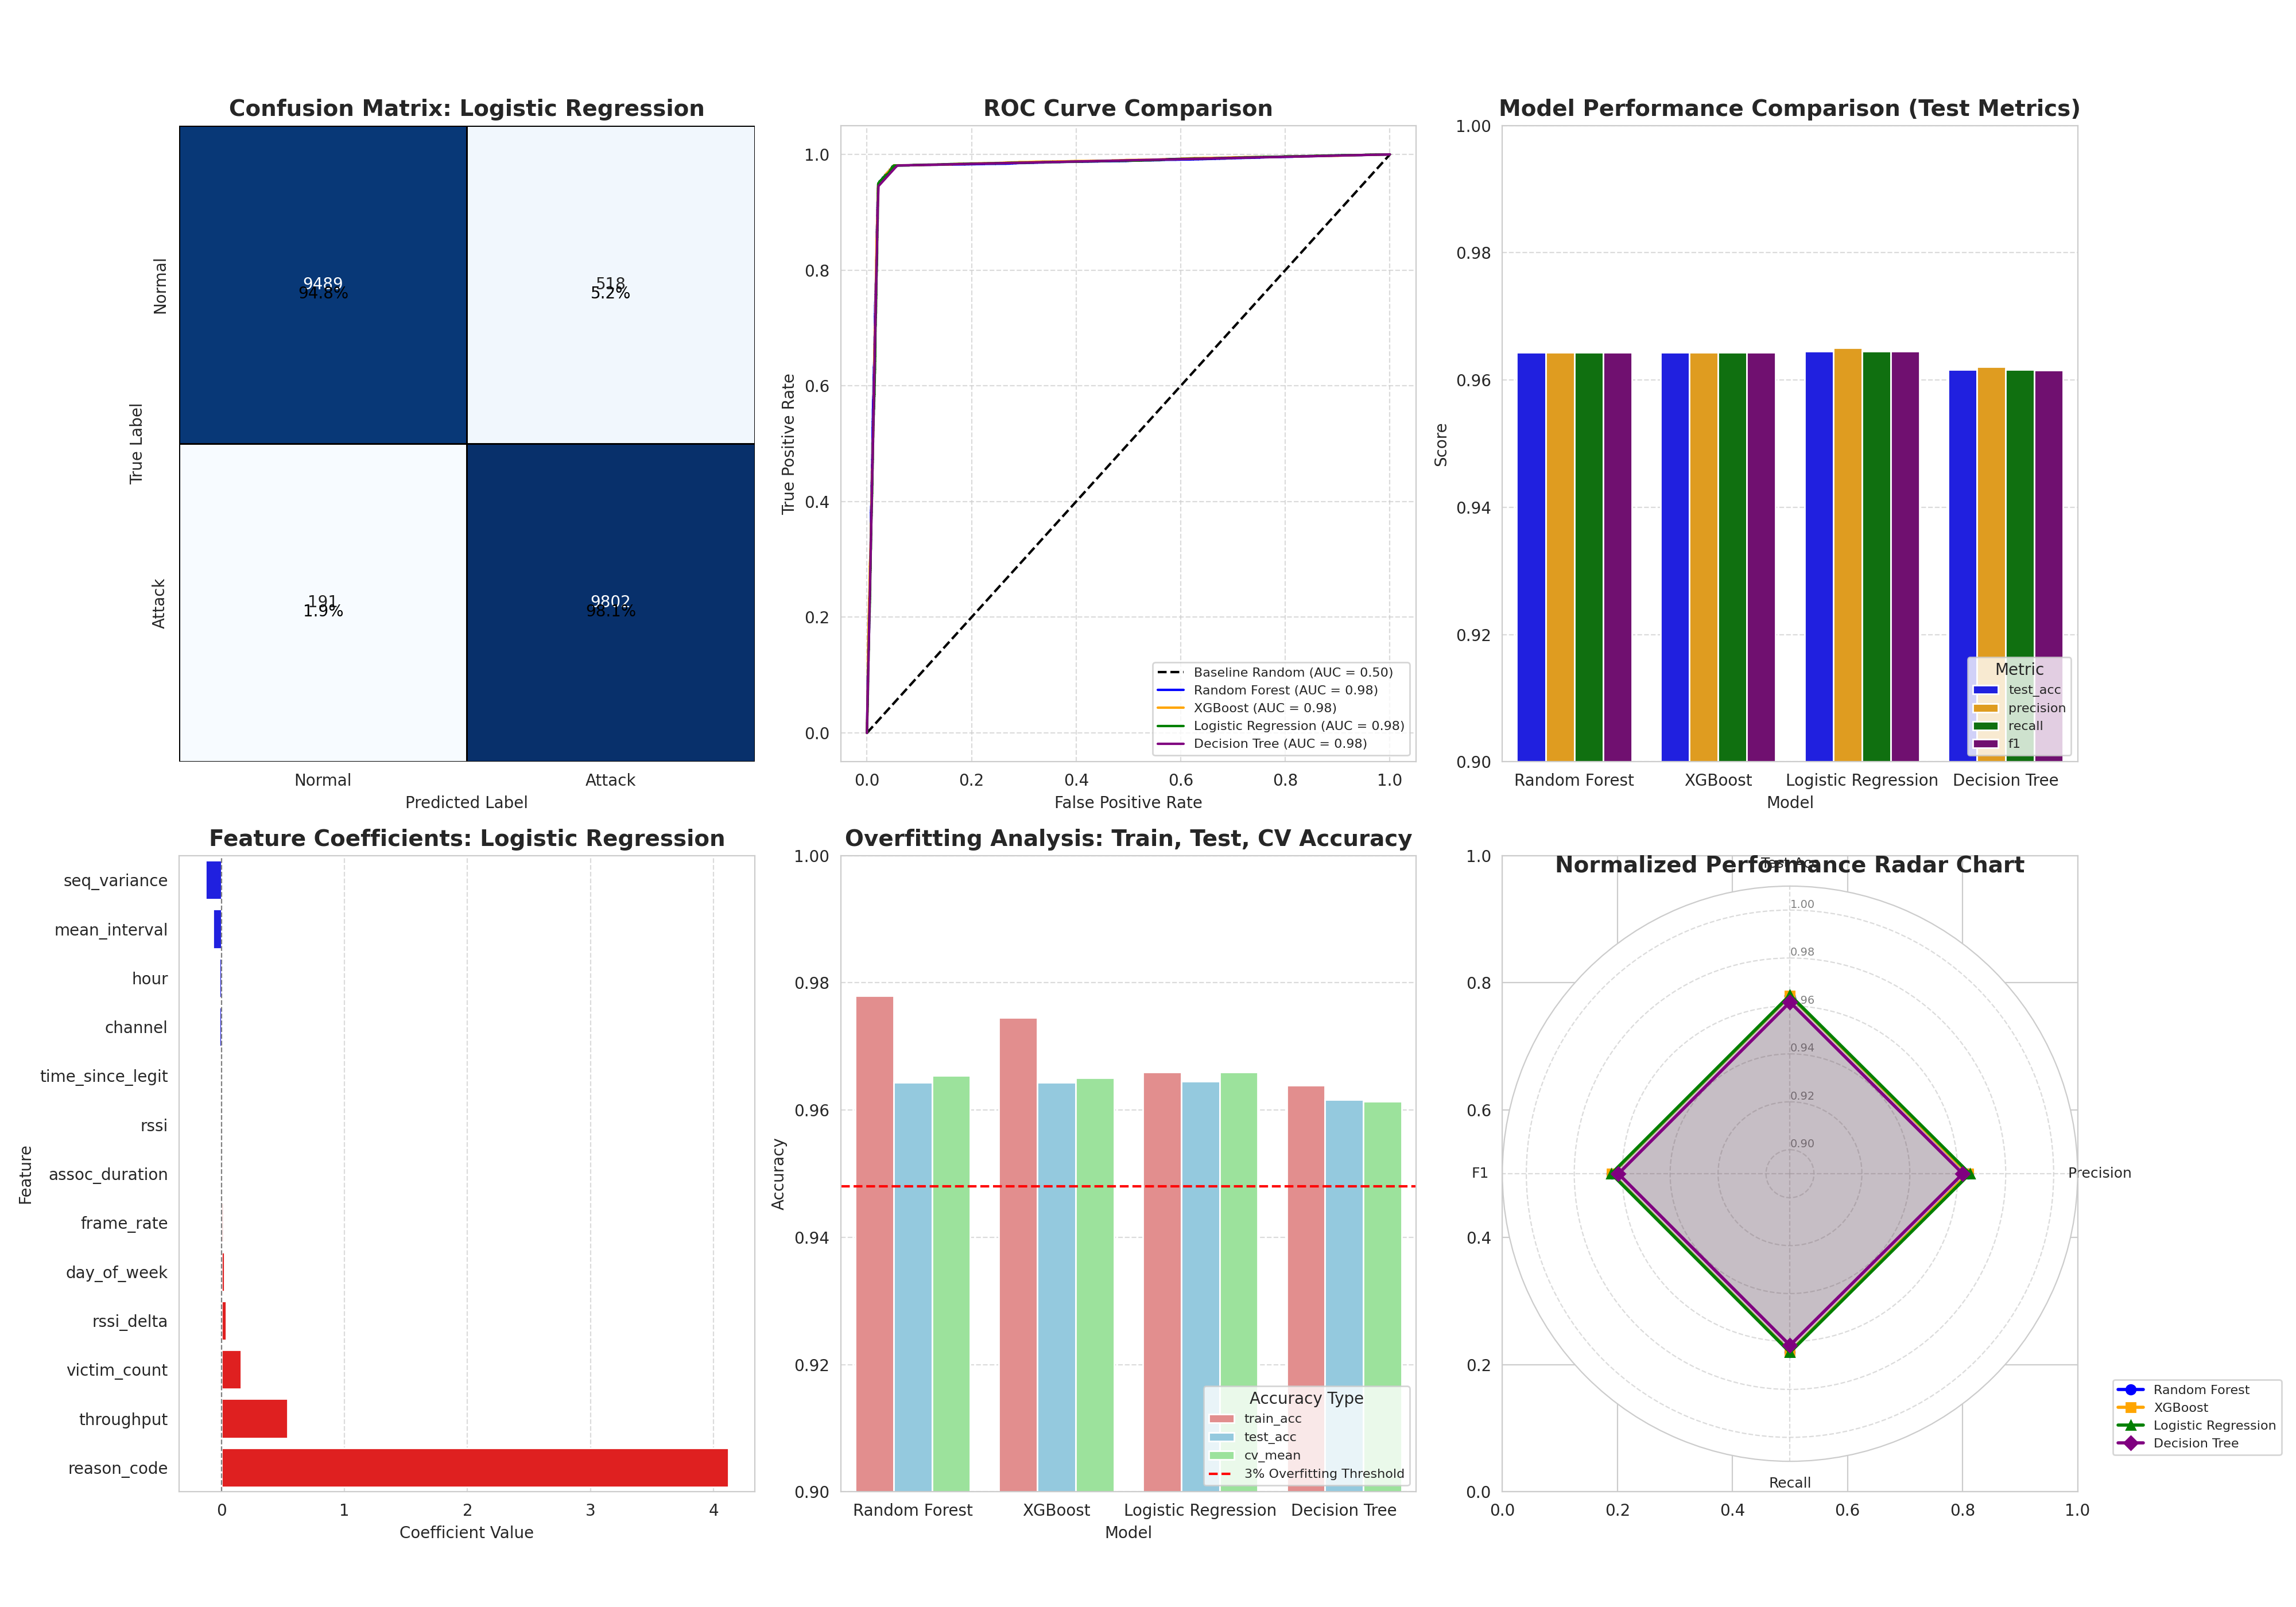
\includegraphics[width=\columnwidth]{final_dashboard.png}
\caption{ML pipeline dashboard: metrics, ROC, feature importance, confusion matrices, overfitting analysis.}
\label{fig:dashboard}
\end{figure}

% ── 7. CONCLUSION ────────────────────────────────────────────
\section{Conclusion}

This paper presented a real-time Wi-Fi deauthentication detection and prevention system with three parallel detection layers and autonomous four-level defense. The system achieves 96.5\% accuracy, sub-500ms latency, and sub-200ms victim reconnection without MAC blocking. Future work includes multi-channel monitoring, larger real-world datasets, WPA3 testing, and eBPF/XDP acceleration.

% ── REFERENCES ───────────────────────────────────────────────
\begin{thebibliography}{14}

\bibitem{ieee80211}
IEEE, ``IEEE Std 802.11-2020,'' 2020.

\bibitem{aireplayng}
Aircrack-ng, ``Aireplay-ng,'' \url{https://www.aircrack-ng.org/}, 2024.

\bibitem{mdk4}
MDK4, \url{https://github.com/aircrack-ng/mdk4}, 2023.

\bibitem{vanhoef2017}
S.~Vanhoef and F.~Piessens, ``Key Reinstallation Attacks,'' \emph{ACM CCS}, 2017.

\bibitem{kismet}
Kismet, \url{https://www.kismetwireless.net/}, 2024.

\bibitem{waidps}
Waidps, \url{https://github.com/SYWorks/waidps}, 2014.

\bibitem{bellardo2003}
J.~Bellardo and S.~Savage, ``802.11 DoS Attacks,'' \emph{USENIX Security}, 2003.

\bibitem{wpa3spec}
Wi-Fi Alliance, ``WPA3 Spec v3.0,'' 2020.

\bibitem{arbaugh2002}
W.~Arbaugh et al., ``Your 802.11 Network Has No Clothes,'' \emph{IEEE Wireless Commun.}, 2002.

\bibitem{aminanto2018}
M.~Aminanto et al., ``Deep Abstraction for Wi-Fi Impersonation Detection,'' \emph{IEEE TIFS}, 2018.

\bibitem{btoush2024}
A.~Btoush, ``Real-Time Detection of 802.11 Deauth Attacks,'' \emph{JNCA}, 2024.

\bibitem{danev2012}
B.~Danev et al., ``Physical-Layer Identification,'' \emph{ACM Comp. Surveys}, 2012.

\bibitem{jana2010}
S.~Jana and S.~Kasera, ``Unauthorized AP Detection via Clock Skews,'' \emph{IEEE TMC}, 2010.

\bibitem{scapy}
P.~Biondi, ``Scapy,'' \url{https://scapy.net/}, 2024.

\end{thebibliography}

\end{document}
